%
% fig/quadtree.tex -- Quadtree-Unterteilung (3 Stadien)
%
% Nachbau der SVG-Abbildung: Startquadrat -> Vierteln & Zaehlen -> Verfeinern
%
\begin{figure}
\centering
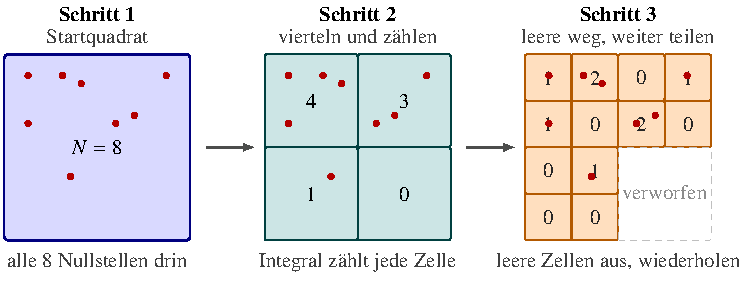
\includegraphics{papers/weyl/images/quadtree.pdf}
\caption{Drei Stadien von Weyls Algorithmus an einem Beispielpolynom mit $8$ Nullstellen.
Links das Startquadrat $D = [-r,r] \times [-r,r]$, das alle Nullstellen umschliesst.
Mitte: nach der ersten Iteration ist $D$ in vier Teilquadrate zerlegt, das
Wegintegral liefert die Nullstellenanzahl jedes Teilquadrats; in unserem Beispiel
$4$, $3$, $1$ und $0$ --- die Probe $4+3+1+0 = 8$ stimmt.
Rechts: das leere Quadrat (unten rechts) wird verworfen, die übrigen drei werden
ihrerseits geviertelt. Der Prozess wiederholt sich, bis jede Nullstelle in einem
eigenen kleinen Quadrat isoliert ist.
\label{weyl:fig:quadtree}}
\end{figure}
